%\documentclass[review]{cvpr}
\documentclass[final]{cvpr}

%\usepackage{cvpr}
\usepackage{times}
\usepackage{epsfig}
\usepackage{graphicx}
\usepackage{amsmath}
\usepackage{amssymb}
\usepackage{subfigure}
\usepackage{overpic}
\usepackage{diagbox}
\usepackage{enumitem}
\setenumerate[1]{itemsep=0pt,partopsep=0pt,parsep=\parskip,topsep=5pt}
\setitemize[1]{itemsep=0pt,partopsep=0pt,parsep=\parskip,topsep=5pt}
\setdescription{itemsep=0pt,partopsep=0pt,parsep=\parskip,topsep=5pt}

% Include other packages here, before hyperref.

% If you comment hyperref and then uncomment it, you should delete
% egpaper.aux before re-running latex.  (Or just hit 'q' on the first latex
% run, let it finish, and you should be clear).
\usepackage[pagebackref=true,breaklinks=true,colorlinks,bookmarks=false]{hyperref}


%\cvprfinalcopy % *** Uncomment this line for the final submission

\def\cvprPaperID{1} % *** Enter the CVPR Paper ID here
\def\confYear{CVPR 2020}


\newcommand{\cmm}[1]{\textcolor[rgb]{0,0.6,0}{CMM: #1}}
\newcommand{\todo}[1]{{\textcolor{red}{\bf [#1]}}}
\newcommand{\alert}[1]{\textcolor[rgb]{.6,0,0}{#1}}

\newcommand{\IT}{IT\cite{98pami/Itti}}
\newcommand{\MZ}{MZ\cite{03ACMMM/Ma_Contrast-based}}
\newcommand{\GB}{GB\cite{conf/nips/HarelKP06}}
\newcommand{\SR}{SR\cite{07cvpr/hou_SpectralResidual}}
\newcommand{\FT}{FT\cite{09cvpr/Achanta_FTSaliency}}
\newcommand{\CA}{CA\cite{10cvpr/goferman_context}}
\newcommand{\LC}{LC\cite{06acmmm/ZhaiS_spatiotemporal}}
\newcommand{\AC}{AC\cite{08cvs/achanta_salient}}

\newcommand{\HC}{HC-maps }
\newcommand{\RC}{RC-maps }
\newcommand{\Lab}{$L^*a^*b^*$}

\newcommand{\vnudge}{\vspace*{-.1in}}
%\newcommand{\vnudge}{\vspace*{-2pt}}

\newcommand{\mypara}[1]{\paragraph{#1.}}

%\renewcommand{\baselinestretch}{0.995}


\graphicspath{{figures/}}

% Pages are numbered in submission mode, and unnumbered in camera-ready
%\ifcvprfinal\pagestyle{empty}\fi
\setcounter{page}{1}

\begin{document}

%%%%%%%%% TITLE

\title{Mid-Term Report for Final Project Gomoku}
\author{Zhi-Jie Zhang\ 18307130184\quad \quad  Wen-Bo Du\ 18307110359 \\
    {\tt \small December 8$^{th}$, 2020 Fall}
}

\maketitle
% \thispagestyle{empty}

%%%%%%%%% ABSTRACT
\begin{abstract}
%
We implemented a Gomoku AI by using adversarial game tree search with $\alpha$-$\beta$ pruning. 
%
In details, a score function is used to score all points on the board, and update the scores dynamically to evaluate the current importance on each point for both players, which helps the AI to understand the board state and give the AI strategy to choose its next move.
%
Besides, because a deeper search usually means a better move choice but a longer search time, we add some heuristic information and use some greedy strategy to obtain reductions to speed up the process of game tree search, which lets the AI achieve a deeper search and makes it think not only quicker but also smarter.
%
And to speed up the minimax search process further, we introduced a data structure named $Zobrist\ Table$, and optimized the code implement, which also improves the AI a lot.
%
Finally by now, we can do minimax search with depth 6 no more than 10 seconds one step in average, and got at most 1353 rating under Bayesian Elo.
\end{abstract}




%%%%%%%%% BODY TEXT %%%%%%%%%%%%%%%%%%%%%%%%%%%%%%%%%%%%%%%%
\section{Introduction}\label{sec:Introduction}

Gomoku is a board game that originated from one of the
various kinds of black and white chess games in ancient China.
%
Nowadays, it has become a popular game played in many places
of the world. A sufficient amount of black or white pieces are
offered to each player. 
%
The players in turns place one piece on the
board. 
%
The winner is the first who forms a line of at least five
adjacent pieces of his color, in horizontal, vertical or diagonal
directions on the board. 
%
Such winning line is called five-in-a-row
which is also referred to the name of the game Gomoku.  

The most classic algorithms of playing Gomoku is the minimax search algorithm.
%
A minimax algorithm is a recursive algorithm 
for choosing the next move in turn. 
%
A value associated with each state of the game is provided, 
which indicates how good it would be for the player to reach such state.
%
The player then makes the move that maximizes the minimum value 
of the position resulting from the opponent's possible following moves.
%
It is perfect to reach a winning state, however, Gomoku has high
complexity with such simple rules, 
and a winning state may not be possible to search so deep to reach.
%
Therefore, cutting off in a certain depth and a effective evaluate function is needed.
%

However, as William said \cite{91ieee/wt},a complete search to a depth of $n$ moves 
requires evaluations of $p!/(p-n)!$ board situations, where $p$ is the 
current number of legal moves. 
%
Fortunately, the $\alpha-\beta$ pruning has been developed
to speed up minimax tree search. 
%
It stops evaluating a move when at least one possibility
has been found that proves the move to be worse than a previously examined move. 

Besides, more techniques are applied to speed up further.
%
To make $\alpha-\beta$ more effective, the search order is dynamically determined according to a heuristic function. 
%
We take accurate and approximate reductions as well. 
%
Accurate reductions make the AI agent be able to react under some specific situation and approximate reductions allowed the AI agent only consider Top-B "most important" children nodes. 
%
In addiction, Zobrist hashing is used to avoid analyzing the same state more than once. 
\\
\\
\noindent Organization for the following report:
\begin{itemize}
\item Section 2: \textbf{Point Score and Evaluation}
\item Section 3: Minimax with Alpha-Beta Pruning
\item Section 4: Accurate and Approximate Reductions
\item Section 5: Zobrist Table
\item Section 6: Code Optimization
\item Section 7: Experimental Comparisons
\end{itemize}

%%%%%%%%%%%%%%%%%%%%%%%%%%%%%%%%%%%%%%%%%%%%%%%%%%%%%%%%%%
\section{Point Score and Evaluation}\label{sec:Evaluation}

\mypara{$Point\ Score$}
To choose a good move, it is needed to let the agent understand a fixed state, and know which points are good for itself, and which points are good for its enemy.
%
To realize this, a score function is developed, which gives each point two scores: one for black player, another for white player.
%
For a point already filled with black chess, its white score equals to 0 and it has a positive black score, vice versa.
%
And for a point empty, its white score and black score are both positive.
%
As for how high the score is, it depends on the importance of this point for either black or white, and the degree of importance is measured by the specific chess shapes, for example, 'live three', 'sleep four', etc.
%
Each shape of the chess has a fixed score, and a score for a fixed point is calculated by the mixture of four directions: $r$ (row), $c$ (column), $m$ (main diagonal) and $v$ (vice diagonal).
%
\par In practice, we consider 9 types of chess shape: $live one$, $live two$, $live three$, $live four$, $sleep one$, $sleep two$, $sleep three$, $sleep four$, and $five$. And give them score as follows:
%
\begin{table}[!htbp]
\centering
\label{table1} 
\scalebox{1.1}{
\begin{tabular}{|c|c c c c c|}
\hline
&one&two&three&four&five\\
\hline
live&$10$ &$10^2$ &$10^3$&$10^5$&$10^7$\\
sleep&$1$ &$10$ &$10^2$&$10^4$&$10^7$\\
\hline
\end{tabular}}
\caption{Scores for different chess shape} 
\end{table}\\
%
\begin{figure}[h]
\centering 
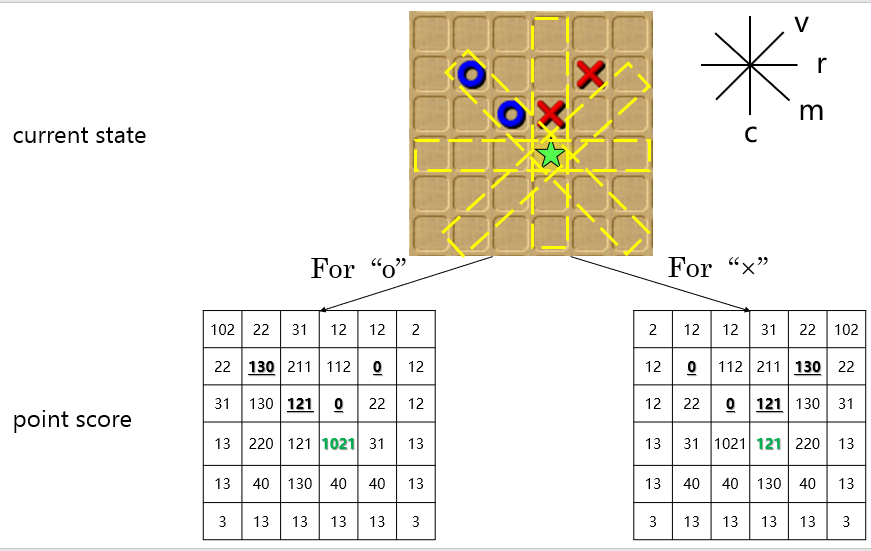
\includegraphics[width=0.43\textwidth]{figures/pic1.png} 
\caption{A simple example of how score function works} 
\label{Fig.main1} %用于文内引用的标签
\end{figure}
%

\noindent Fig.\ 1 is a illustrative example on a small 6×6 board. 
%
The score function will give each point on the current board two scores for both player o and player ×.
%
And for instance, when scoring the star point, which is empty currently, this point's score for player o is: 
\begin{align*}
    s_o &= s_o(r) + s_o(c) + s_o(m) + s_o(v) \\
    &= s(live\ 1)+s(sleep\ 1)+s(live\ 3)+s(live\ 1) \\
    &= 10 + 1 + 1000 + 10 \\
    &= 1021
\end{align*}
The score for player × can be calculated similarly: 
\begin{align*}
    s_x &= s_x(r) + s_x(c) + s_x(m) + s_x(v) \\
    &= s(live\ 1)+s(live\ 2)+s(sleep\ 1)+s(live\ 1) \\
    &= 10 + 100 + 1 + 10 \\
    &= 121
\end{align*}



%%%%%%%%%%%%%%%%%%%%%%%%%%%%%%%%%%%%%%%%%%%%%%%
\vnudge
\mypara{$State\ Evaluation$} When it is necessary to evaluate a fixed board state, the AI will traverse all the points that have been placed by black chess to get whole-score for player 1, and do the same for the white chess to get whole-score for player 2, then the value of board is a combination of two whole-scores:
$$v = s_1 - r\cdot s_2$$
%
\par In the formula above, $s_1$ is the whole-score for the agent,  while $s_2$ is the whole-score for its enemy, and the result $v$ is the value used to evaluate the situation our agent is facing: the higher $v$ means the better situation.
%
And as is all known, in board games, the same board state don't mean the same situation for a fixed player yet, because it should be considered whether the player is on first hand or not under the current state .
%
So the multiplier $r$ is introduced to check either the agent is on first hand or second hand under the current board state.
%
If the agent is on first hand, its own score matters more, so we set $r < 1$ in this case; else if the agent is on second hand, its enemy will move first, then its enemy's score matters more, so we set $r > 1$.
%
In practice, we set $r = 1.05$ when the agent is on first hand, and $r = 0.95$ when its enemy is on first hand.

%%%%%%%%%%%%%%%%%%%%%%%%%%%%%%%%%%%%%%%%%%%%%%%%%%%%%%%%%%
\section{Minimax with Alpha-Beta Pruning}
\label{sec:Minimax}
The algorithm maintains two values, alpha and beta, which respectively represent the minimum score that the maximizing player is assured of and the maximum score that the minimizing player is assured of. 

Initially, alpha is negative infinity and beta is positive infinity, 
i.e. both players start with their worst possible score.
Whenever the maximum score that the minimizing player (i.e. the "beta" player) 
is assured of becomes less than the minimum score that the maximizing player 
(i.e., the "alpha" player) is assured of (i.e. beta < alpha), the maximizing player need not consider further descendants of this node, as they will never be reached in the actual play.

\begin{figure}[h]
\centering 
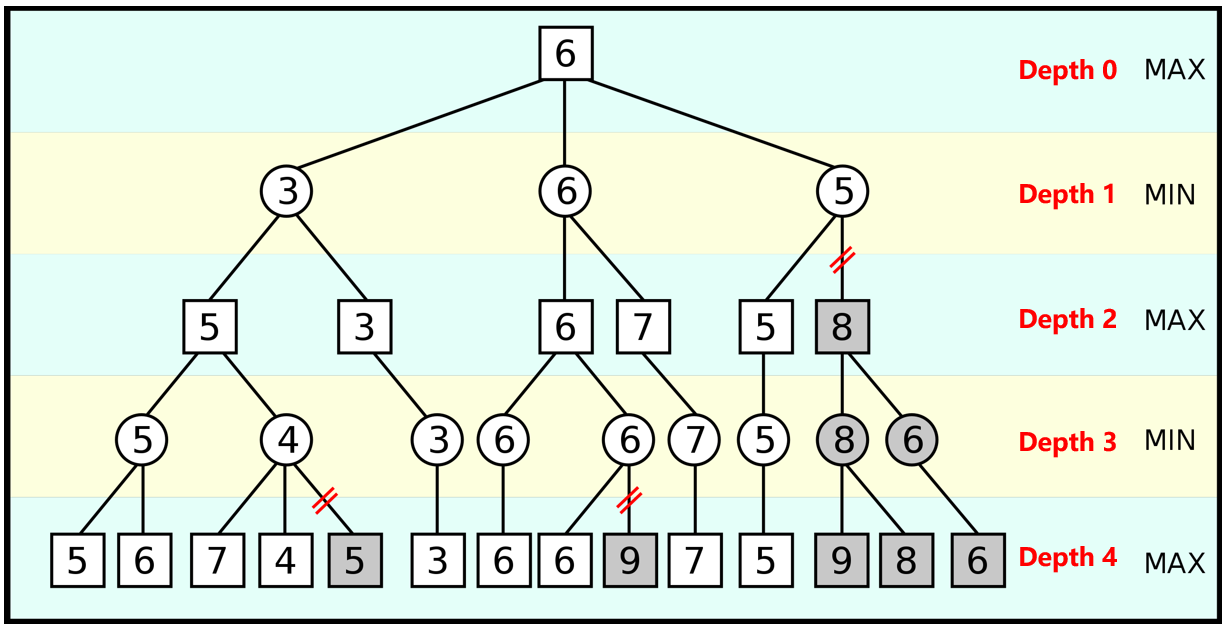
\includegraphics[width=0.43\textwidth]{figures/pic7.png} 
\caption{alpha-beta pruning} 
\label{Fig.main1} %用于文内引用的标签
\end{figure}

\par As is showed in Fig. 2, in practice, if we want the agent search at most 4 depth, then the agent would cut off the tree search and evaluate the board at $Depth\ 4$ in Fig. 2. And if we want the agent search at most 3 depth, then we will cut the tree and evaluate the board at $Depth\ 3$ in Fig. 2. When evaluate, we will use the formula mentioned before: $v = s_1 - r\cdot s_2$, and set $r = 1.05$ for $Depth\ 4$ and $r = 0.95$ for $Depth\ 3$, remark it depends on whether the agent is first hand or not.

%%%%%%%%%%%%%%%%%%%%%%%%%%%%%%%%%%%%%%%%%%%%%%%%%%%%%%%%%%
\section{Accurate and Approximate Reductions}\label{sec:AD}
For the tree searching algorithm, "the 
depth of search can always be a bottleneck". \cite{adp/ztt}
%
Although the $\alpha-\beta$ pruning is effective, it is not effective enough.
%
Accurate and approximate reductions is induced to shrink the search space of the game tree,
in order to imply a deeper search.
%
It is one of the important reason that our best version of AI agent could finish the search of 6 or 7 depth without timeout.
%

\subsection{Accurate Reductions} 
Accurate reductions is the reductions that prune some of the branches on the tree without loss of the quality of the result. 
%
It happened under some special situations.
%

\begin{figure}[htbp]
\centering 
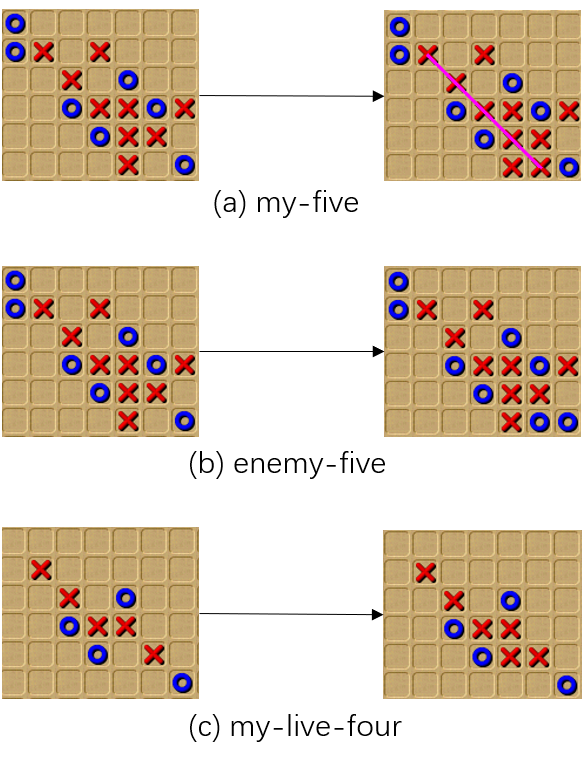
\includegraphics[width=0.35\textwidth]{figures/pic5.png} 
\caption{Accurate Reduction} 
\label{Fig.main2} %用于文内引用的标签
\end{figure}

Three are three situations that the best move is so clear that the AI agent can choose it directly without searching any more.
%

(a) my-five

If there is a move that be able to construct a five-in-a-row of mine, the AI agent can choose it and win the game. Clearly, such move is the best move on the state.

(b) enemy-five

If there is not a move that be able to construct a five-in-a-row of mine,
which mean the AI agent cannot win the game immediately, then he need to think about its enemy. If there is a move that be able to construct a five-in-a-row of enemy, the AI agent must choose it or he would lose the game immediately. Therefore, such move is the best move.

(c) my-live-four

If there is not a move that be able to construct a five-in-a-row, mine or enemy, which mean both the two players cannot win in one step,then the AI could consider to win the game in two steps. If there is a move that construct a live-four, the AI agent can choose it and win the game. Such move is the best move as well.

\subsection{Approximate reductions}
%
Approximate reductions is the reductions shrink the search space sharply but without the guarantee that the result is as good as before.
%
The idea of approximate reductions is that the moves considered best in deep depth would be also considered not bad in just 1-depth in institution.(but we don't know how reliable this belief is)
%

Thus, the AI agent could scoring all the possible moves in 1-depth first (yes, that is the point score), and then choose the Top-B moves for deeper searching.
 (Fig. 4)
%

By this way, the branch factor of the search tree would be shrunk from $p$ to $b$, where the $p$ is the legally move positions and the $b$ is a super parameter given.

%
Since $p \gg b$, the search space is weight smaller than the original one.
\begin{figure}[htbp]
\centering 
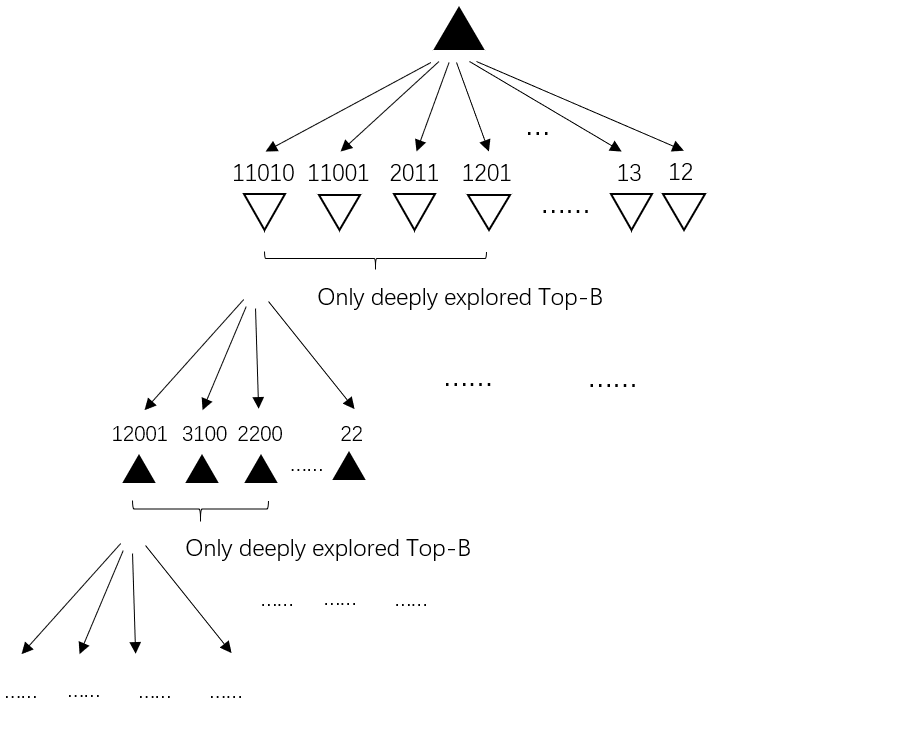
\includegraphics[width=0.45\textwidth]{figures/pic6.png} 
\caption{Approximate Reduction} 
\label{Fig.main3} %用于文内引用的标签
\end{figure}

\mypara{$Adaptive\ Branch\ Factor$}

Empirically, the branch factor of shallow layer should be larger and the branch factor of deep layer can be smaller.
%
For shallow layers, it takes higher risk to exclude a branch - it may cause larger bias on the decision.
%.

In practice, Adaptive Branch Factor is applied that the branch factor would be getting smaller with the search layers getting deeper.

%%%%%%%%%%%%%%%%%%%%%%%%%%%%%%%%%%%%%%%%%%%%%%%%%%%%%%%%%%
\section{Zobrist Table}
As Fig. 5 shows, there are two paths in the $\alpha-\beta$ searching tree.
%
Although the pieces are placed in different position in different turn, 
the two paths reach at the same board state finally.
%
It is the board state that matters in the evaluate function.
%
Therefore, the calculation of the same board state is unnecessary.
%
We shall make use of the value has been calculating before.

\begin{figure}[htbp]
\centering 
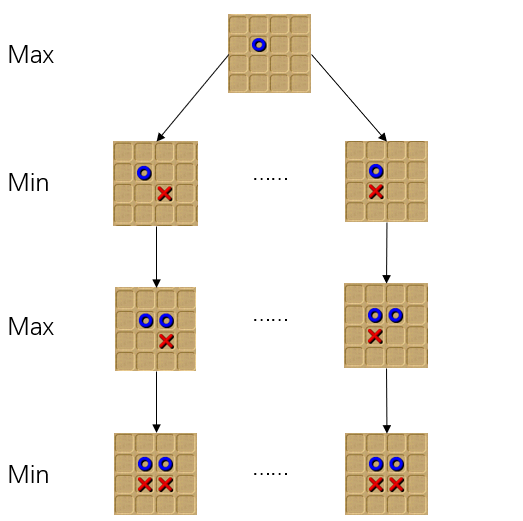
\includegraphics[width=0.45\textwidth]{figures/pic2.png} 
\caption{An example of reaching the same state} 
\label{Fig.main4} %用于文内引用的标签
\end{figure}

Zobrist hashing is invented by and named for Albert Lindsey Zobrist. 
%
It is a hashing construct that widely used in playing board game,
make it easy and effective to detect same board state.
%

Zobrist hashing starts by randomly generating bitstrings for each possible on the board game for each color, 
i.e. for Gomoku, there are 20 $\times$ 20 points and 2 colors.
%
The starting state of the board will be assigned a random bitstrings as well.
%
The length of our implementation is 64.
%

Once a player place a piece on the board. The Zobrist hash is updated by combining the current hash and the bitstring using bitwise XOR. The piece placed could be withdrawn by using bitwise XOR with the bit string again.
%

Since the bitstrings are long enough, different board positions will almost certainly hash to different values.
%
During the $\alpha-\beta$ tree search, 
the values of each state checked are stored in a dictionary with the Zobrist hashing as key.
%
Before calculating the value of a state, we check whether a same state has been checked in the dictionary.
%
Therefore, the calculation of the same board state can be avoided.

%%%%%%%%%%%%%%%%%%%%%%%%%%%%%%%%%%%%%%%%%%%%%%%%%%%%%%%%%%
\section{Code Optimization}
\subsection{Fast Update}
%
After one piece is placed by a player, 
not the whole board but only part of the board is influenced.
%
It is not necessary to scan the whole board and compute the value from scratch.
%
We can just update the score based on the existing results 
and speed up the process.
%

\mypara{$Point\ Update$}
%
Figure 3 shows which point scores would be changed after one more piece is placed. 
%
Only the points in the 
" {\ooalign{$\times$\cr\hidewidth$+$\hidewidth\cr}} "
shape of the placed position will be influenced.

%
In practice, instead of scanning the whole board,
we only update the score of points in the "
{\ooalign{$\times$\cr\hidewidth$+$\hidewidth\cr}} "
shape, and remain the score of other point.

\begin{figure}[htbp]
\centering 
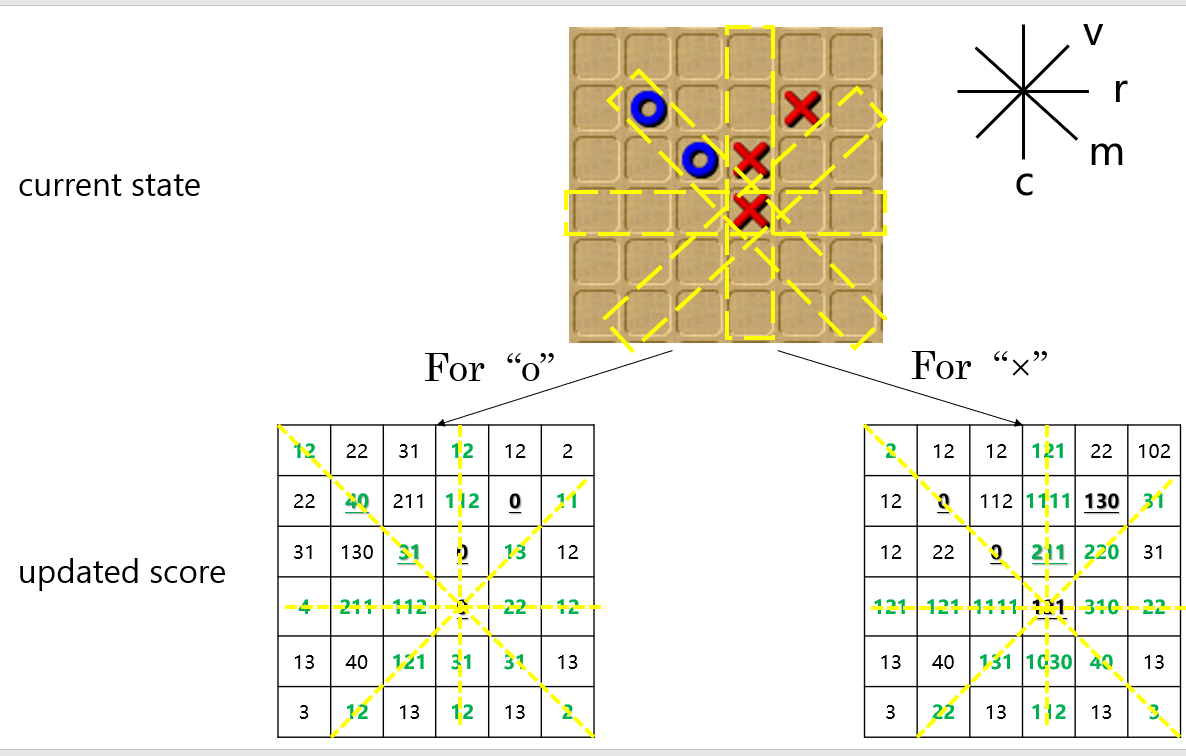
\includegraphics[width=0.45\textwidth]{figures/pic3.png} 
\caption{An example of point update} 
\label{Fig.main5} %用于文内引用的标签
\end{figure}

\mypara{$Direction\ Update$}
%
As mentioned in Section 2, a score for a fixed point is calculated by the mixture of four directions.
%
When the point is influenced and its score need to be updated, 
it is only one of the four directions changed.
%
-- apparently, the position placing the new piece cannot exist in two direction at the same time.

%
For example in Figure 4(a), after the player $\times$ placing one $\times$ pieces, 
the score of star point is clearly affected. 
%
When re-scoring the star point,
it would have had to calculate the score in four direction and then add them up.
%
However, it is actually only the score of $r$ direction (the green one) is changed 
and the computation of three other direction is just waste.
%

In practice, not only the point score but also the point score of each direction would be cached. 
%
By this way, the AI agent is allowed to updated the point score by updating the point score of just one direction.

\begin{figure}[htbp]
\centering 
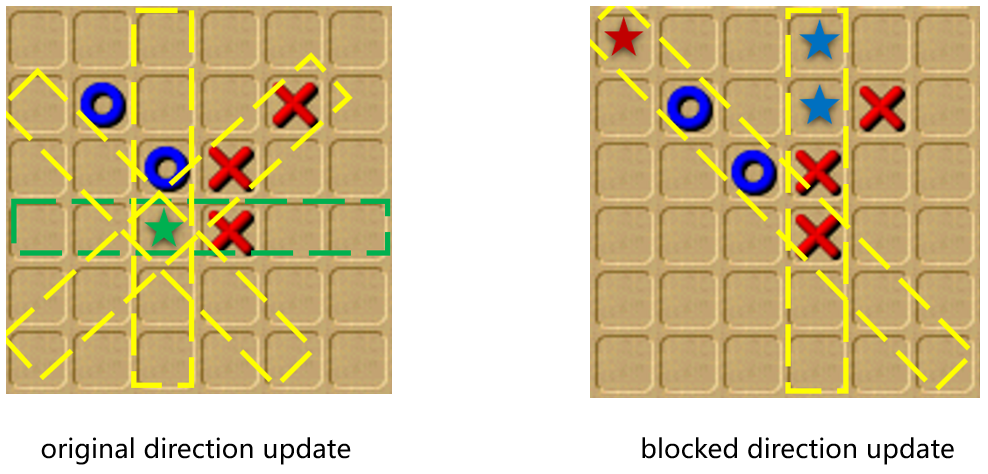
\includegraphics[width=0.4\textwidth]{figures/pic4.png} 
\caption{(a)A schematic for original (b)blocked direction update} 
\label{Fig.main6} %用于文内引用的标签
\end{figure}


\mypara{$Blocked\ Direction\ Update$}
%
In the $20 \times 20$ board, the length of one direction of the 
" {\ooalign{$\times$\cr\hidewidth$+$\hidewidth\cr}} "
should be no less than 9 to count all the possible chess shape.
%
To make it even more faster, the technique of \textbf{Blocked\ Direction\ Update} (BDU) is induced.
%
As the observation of Figure 4(b), for the two blue star point, 
the point scores for $o$ are not changed and similarly for the red star point, 
the point scores for $\times$ are not changed.
%
That is because that there has been already one opponent piece between such point and the newly placed piece.
%
We call such one opponent piece a "Block" that it blocks the influence of the piece.
%

%
In practice, the BDU algorithm scan the
" {\ooalign{$\times$\cr\hidewidth$+$\hidewidth\cr}} "
from the center (the position of newly placed piece). 
%
If it meets a $\times$ piece, the score for $o$ need not to be scanned and updated any more, vice versa.

\subsection{Shared Board}
Logically, each node of the $\alpha-\beta$ search tree should be a state of the board.
%
However, generate a board and store it in each node is both space cost (A board size for each node) and time cost (the deepcopy itself takes time).
%
Since the $\alpha-\beta$ tree searching is a Depth-First-Search(DFS), it is possible to reuse space of a game board. Due to there is only one piece difference between the parent and the child, the reusing will be effective.
%
Two operations is defined:
%

\textbf{Gomoku move(x, y, role)}:
Gomoku moves means a role ($\times$ or $o$) piece is placed in position (x, y). 
%
\begin{itemize}
\item First, update the board state (x, y) to role ($\times$ or $o$)
\item Second, update the score board for $\times$ and $o$ with BDU algorithm
\item Last, update the zobrist of the current board.
\end{itemize}

\textbf{Withdraw move(x, y)}:
Withdraw a move in position (x, y).
\begin{itemize}
\item First, update the board state (x, y) to empty (0)
\item Second, restore the score board for $\times$ and $o$ with BDU algorithm
\item Last, restore the Zobrist of the current board.
\end{itemize}

When the searching algorithm reach to a node, calling Gomoku move to update the board, 
and calling Withdraw move when the subtree of that node has finished search.



%%%%%%%%%%%%%%%%%%%%%%%%%%%%%%%%%%%%%%%%%%%%%%%%%%%%%%%%%%%%%%%%%%%%%%
\section{Experimental Comparisons}\label{sec:Experiment}

\par The experiment consists of two parts, one is the comparison among some different search depth, another is the speed improvement after our code optimization.


\begin{figure}[h]
\centering 
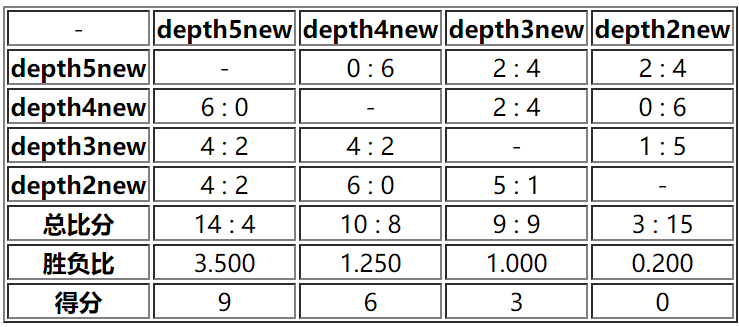
\includegraphics[width=0.45\textwidth]{figures/pic8.png} 
\caption{A comparison among different search depth } 
\label{Fig.main1} %用于文内引用的标签
\end{figure}
\begin{figure}[h]
\centering 
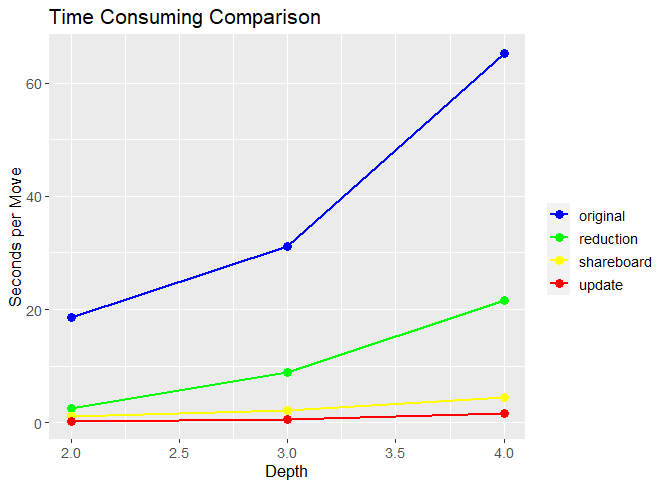
\includegraphics[width=0.5\textwidth]{figures/pic9.png} 
\caption{A time consuming comparison} 
\label{Fig.main1} %用于文内引用的标签
\end{figure}



\par Fig. 8 shows clearly that deeper we search, more wins the agent will get. The AI agent can always beat his siblings with less search depth.

\par Meanwhile, Fig. 9 is a figure that record per-move time cost for different agent editions in one game (with baseline: fiverow), which shows that after adding different code optimization, the Gomoku agent becomes more and more faster.




%%%%%%%%%%%%%%%%%%%%%%%%%%%%%%%%%%%%%%%%%%%%%%%%%%%%%%%%%%%%%%%%%%%%%%
\section{Conclusions and Future Work}\label{sec:Conclusion}

We implement minimax game tree search with $\alpha-\beta$ pruning to realize a Gomoku agent, and achieve a good result.
%
By using some reductions, adding $zobrist\ table$ and optimizing the code, the agent can achieve a depth-7 search quickly by now, which achieves 1353 rating under Bayesian Elo.

But the score for the chess shapes is not as good as we expected, and in real game, the shapes of the chess are much more complex than we have considered.
%
Also, more continuously heuristic information can be add, which is called $checkmate$ in board games.
%
So there still exists a lot of space for improvement.

In future, we can optimize the Gomoku AI further in following aspects:
\begin{itemize}
\item $Checkmate\ and \ threat\ sequence\ search$

\par Checkmate is a terminology for a lot of board games, which means your enemy does a move which you have to respond and take defensive measures, otherwise you will lose the game. 
%
In Gomoku, the existing of multiple checkmates makes it possible to appear must-win situation, double live three is such an example.
%
A winning threat sequence for a player is a action sequence which consists of a sequence of checkmate which leads to a must-win situation\cite{threat}.
%
If such a winning threat sequence exists in a fixed board state, we simply do moves in that sequence and can get a win.
%
So it'll improve the AI a lot if we add such threat sequence search for the current board state.
\item $Improve\ chess\ shape\ score$

\par In the score function by now, it still has some disadvantages because it may make some wrong judgment.
%
For example, under the existing scoring system, a point that can form a double-live-three chess shape can only get score 2000, smaller than a sleep four (score 10000).
%
But if we only consider this, sometimes we will miss other good moves.
%
So it is a time consuming work to design a reasonable scoring system for different chess shapes. 

\item $Use\ ADP\ to\ select\ and\ evaluate$
\par Further, we may use some new technology, such as shallow neural network other than human-defined empirical score function to get point score, which is used in brunch selection and board evaluation.
%
Such shallow neural network can be trained by Adaptive Dynamic Programming (ADP), and employing ADP to train the neural network can obtain each point's winning rate for a fixed board state.
%
Therefore, we can use the result from the ADP to score for board points, which may be much more efficient and faster than empirical chess shape analysis.
\end{itemize}


{\small
\bibliographystyle{ieee}
\bibliography{Saliency}
}

\end{document}
